\documentclass[12pt]{article}
\usepackage{graphicx}
\usepackage{amsmath}
\usepackage{mathtools}
\usepackage{gensymb}

\newcommand{\mydet}[1]{\ensuremath{\begin{vmatrix}#1\end{vmatrix}}}
\providecommand{\brak}[1]{\ensuremath{\left(#1\right)}}
\providecommand{\norm}[1]{\left\lVert#1\right\rVert}
\newcommand{\solution}{\noindent \textbf{Solution: }}
\newcommand{\myvec}[1]{\ensuremath{\begin{pmatrix}#1\end{pmatrix}}}
\let\vec\mathbf

\begin{document}
\begin{center}
\section*{CHAPTER 7 - COORDINATE GEOMETRY}

\end{center}
\section*{Excercise 7.1}

Q4.Check whether (5,-2),(6,4) and (7,-2) are the vertices of an isosceles triangle:

\solution
\begin{enumerate}
\item In an Isosceles triangle, If any 2 of the 3 sides of  triangle are be equal then it satisfies the condition.Let us assume the given three points be,
	\begin{align}
\vec{A} , \vec{B} , \vec{C}
	\end{align}
Now, the direction vectors of AB,BC and CA are:
	\begin{align}
	\vec{A} = \myvec{
	    5\\
	   -2\\
		},
	\vec{B} = \myvec{
	    6\\
		4\\
		},
	\vec{C} = \myvec{
		7\\
	   -2\\
	    }
	\end{align}  
	\begin{align}
		\vec{A} - \vec{B} = \myvec{5\\-2} - \myvec{6\\4} = \myvec{-1\\-6}\\
		\vec{B} - \vec{C} = \myvec{6\\4} - \myvec{7\\-2} = \myvec{-1\\6}\\
		\vec{C} - \vec{A} = \myvec{7\\-2} - \myvec{5\\-2} = \myvec{2\\0}		
	\end{align}
	\begin{align}
	(\vec{A}-\vec{B})^\top (\vec{B}-\vec{C}) &= \myvec{-1&-6} \myvec{-1\\6} = 37 \\
	(\vec{B}-\vec{C})^\top (\vec{C}-\vec{A}) &= \myvec{1&6} \myvec{2\\0}   = -2 \\
	(\vec{C}-\vec{A})^\top (\vec{A}-\vec{B}) &= \myvec{2&0} \myvec{-1\\-6} = -2	
	\end{align}
    Therefore,from the above equation we can see that,
	\begin{align}
 {\vec{A} -\vec{B}}\perp {\vec{B} -\vec{C}}\\
	\angle BCA = \angle CAB   
	\end{align}    	
Thus, the given points proves that, it is an Isosceles Triangle.
\begin{figure}[!h]
	\begin{center} 
	    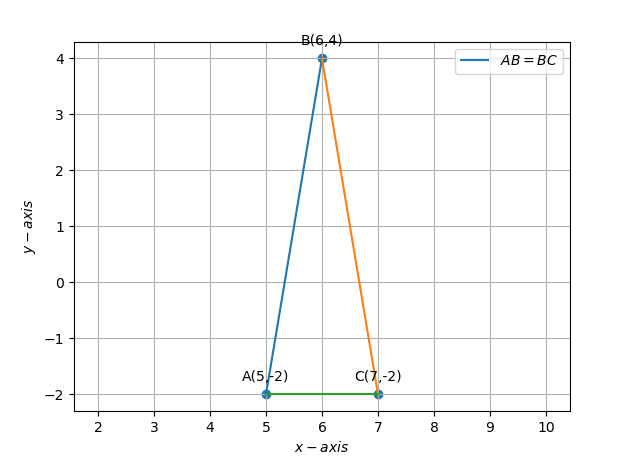
\includegraphics[width=\columnwidth]{figs/Vector2.png}
	\end{center}
\caption{Isoscles Triangle with the given coordinates}
\label{fig:Fig}
\end{figure}
\end{enumerate}
\end{document}
	